%%%%%%%%%%%%%%%%%%%%%%%%%%%%%%%%%%%%%%%%%
% Journal Article
% LaTeX Template
% Version 1.4 (15/5/16)
%
% This template has been downloaded from:
% http://www.LaTeXTemplates.com
%
% Original author:
% Frits Wenneker (http://www.howtotex.com) with extensive modifications by
% Vel (vel@LaTeXTemplates.com)
%
% License:
% CC BY-NC-SA 3.0 (http://creativecommons.org/licenses/by-nc-sa/3.0/)
%
%%%%%%%%%%%%%%%%%%%%%%%%%%%%%%%%%%%%%%%%%

%----------------------------------------------------------------------------------------
%	PACKAGES AND OTHER DOCUMENT CONFIGURATIONS
%----------------------------------------------------------------------------------------

\documentclass[twoside,twocolumn]{article}

\usepackage{blindtext} % Package to generate dummy text throughout this template 

\usepackage[sc]{mathpazo} % Use the Palatino font
\usepackage[T1]{fontenc} % Use 8-bit encoding that has 256 glyphs
\linespread{1.05} % Line spacing - Palatino needs more space between lines
\usepackage{microtype} % Slightly tweak font spacing for aesthetics

\usepackage[english]{babel} % Language hyphenation and typographical rules

\usepackage[margin=2.54cm,top=24mm,columnsep=20pt]{geometry} % Document margins
\usepackage[hang, small,labelfont=bf,up,textfont=it,up]{caption} % Custom captions under/above floats in tables or figures
\usepackage{booktabs} % Horizontal rules in tables

\usepackage{lettrine} % The lettrine is the first enlarged letter at the beginning of the text

\usepackage{enumitem} % Customized lists
\setlist[itemize]{noitemsep} % Make itemize lists more compact

\usepackage{abstract} % Allows abstract customization
\renewcommand{\abstractnamefont}{\normalfont\bfseries} % Set the "Abstract" text to bold
\renewcommand{\abstracttextfont}{\normalfont\small\itshape} % Set the abstract itself to small italic text

\usepackage{titlesec} % Allows customization of titles
\titleformat{\section}[block]{\large\scshape\centering}{\thesection.}{1em}{} % Change the look of the section titles
\titleformat{\subsection}[block]{\large\centering}{\thesubsection.}{1em}{} % Change the look of the section titles



\usepackage{titling} % Customizing the title section

\usepackage{hyperref} % For hyperlinks in the PDF

\usepackage{amsmath}
\usepackage{graphicx}
\usepackage{url}
\usepackage{color}
\usepackage{subcaption}

%----------------------------------------------------------------------------------------
%	TITLE SECTION
%----------------------------------------------------------------------------------------

\setlength{\droptitle}{-4\baselineskip} % Move the title up

\pretitle{\begin{center}\LARGE\bfseries} % Article title formatting
	\posttitle{\end{center}} % Article title closing formatting
\title{Comparing LDA and CCA as a Guide to Improve Automatic Image Description Systems} % Article title
\author{%
	\textsc{Wout Vekemans} \\[1ex] % Your name
	\normalsize KULeuven \\ % Your institution
	\normalsize \href{mailto:w.vekemans@gmail.com}{w.vekemans@gmail.com}
	\and % Uncomment if 2 authors are required, duplicate these 4 lines if more
	\textsc{Thijs Dieltjens} \\[1ex] % Second author's name
	\normalsize KULeuven \\ % Second author's institution
	\normalsize \href{mailto:thijsdieltjens@gmail.com}{thijsdieltjens@gmail.com} % Second author's email address
}
\date{June 3, 2016} % Leave empty to omit a date
\renewcommand{\maketitlehookd}{%
	\begin{abstract}
		\noindent 
		We present a model that generates novel, fluent and grammatically correct image descriptions. Most of the current systems based on recurrent neural networks show the same flaws. The used words are too general and are not related to the picture. The generated sentences are often way shorter than the descriptions a human would provide. The most recent literature tries to solve this first problem by adding additional information into the recurrent neural network. This paper compares two sources of semantic information: Latent Dirichlet Analysis (LDA) and Canonical Correlation Analysis (CCA). We compare their effect on both recurrent neural networks (RNN) and long short-term memory networks (LSTM). Both techniques improve the results. Experiments show that both of these models are able to deal with noisy training data. Adding normalization to the search algorithm used to generate the sentences solves the second problem. A first form of normalization is able to improve results and creates longer sentences. A second normalization function leads to more creative sentences but makes more mistakes. The results of this paper are comparable to the literature, but do not outperform current attention based systems.
	\end{abstract}
}

%----------------------------------------------------------------------------------------

\begin{document}
	
	% Print the title
	\maketitle
	
	%----------------------------------------------------------------------------------------
	%	ARTICLE CONTENTS
	%----------------------------------------------------------------------------------------
	
	\section{Introduction}
	Automatic image description is a complex problem. It combines elements from the domains of both Computer Vision and Natural Language Processing. A captioning system must be able to detect what is in the image, label these objects and combine them in a fluent, grammatically correct sentence. Figure~\ref{fig:exampledescription} shows an example of a correctly described picture.
	
	\begin{figure}[!htb]
		\centering
		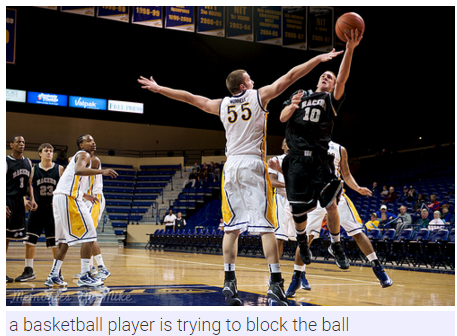
\includegraphics[width=\linewidth]{blocking_the_ball_trimmed.png}
		\caption{Correctly described image}
		\label{fig:exampledescription}
	\end{figure}
	
	The problem is drawing more and more attention from the industry. Internet giant Facebook~\cite{facebook}, for example, is implementing it in their application to aid the visually impaired.
	
	The currently best performing systems contain a convolutional neural network (CNN) that creates an image representation. A recurrent neural network based language model uses this representation as input to generate a description.
	An analysis of existing systems shows that the same mistakes occur in many systems. The generated captions are too short and they do not relate to the image. Jia et al.~\cite{Fernando2015} suggest that this is caused by two opposing forces. The generated caption has to comply with the language model but also has to describe the given image.
	
	We deal with this problem in two ways. The first addition focuses on the lack of relation between images and their generated description. Adding semantic information seems a viable way to guide the generation in the right direction. This information is extracted from the images in two ways. In the first way a model extracts topic distributions with Latent Dirichlet Allocation~\cite{Blei2012}. A second approach uses Canonical Correlation Analysis to project the unseen images into a multimodal image-sentence space. Both methods produce an additional vector which acts as a guide in the language model. Our contribution also compares the resistance to noise in the training data of the two methods.
	
	A second proposed addition normalizes the beam search algorithm that generates sentences based on predicted word probability distributions. Based on Jia et al.~\cite{Fernando2015} we implement their best scoring Gaussian normalization function. They claim this results in longer sentences and achieves better scores on BLEU and Meteor. We introduce a new normalization function based on word frequency in the training set. This leads to more creative and longer sentences. 
	
	The rest of this paper is as follows. First we provide an overview of the most recent works that solve the image description problem in section~\ref{sec:related}. After that, section~\ref{sec:methodology} elaborates on the extraction of semantic information from the images and how this information is added to existing systems. Section~\ref{sec:exp} provides a detailed overview of the conducted experiments and their results. 
	
	\section{Related Work}
	\label{sec:related}
	This section provides an overview of previously proposed image description systems.
	A first type of older systems follows a transfer-based approach. This approach searches for visually similar images and transforms their captions to a sentence describing the image~\cite{Devlin2015a,Hodosh2013,Kuznetsova2012,Ordonez2011}.
	This approach generally produces results that are less natural and creative, and often requires manually constructed rules.
	
	A second type of systems extracts visual features such as object and scene detections and uses them to fill in predefined templates~\cite{Farhadi2010,Mitchell2012,Yang2011}. These models produce new sentences but do not allow for rich enough captions.
	Because of the use of manually constructed rigid templates the generated descriptions also feel less natural. 
	
	Most recently however the task of describing images is often seen as a  ``translation'' from the image to the target language.
	Methods from machine translation are therefore transferred to this problem. The global structure of the system often follows an encoder-decoder framework.
	The best performing works use a convolutional neural network to represent image features. Most methods use the values of the top layer of a pre-trained convolutional neural network as the image representation~\cite{Donahue2015,Mao2014a,Karpathy2015,Google}. Other methods use models such as R-CNN~\cite{Girshick2014} to generate representations for the most important regions of the image~\cite{Jin2015,Mitchell2015}.
	The image representation then serves as an input for a language model.
	Generally two types of language models are proposed. The first type are entropy based language models that also try to couple parts of the image to certain words~\cite{Lebret2015,Mitchell2015}. Most models however use a fully statistical language model based on neural networks~\cite{Kiros2013}. Mao et al.~\cite{Mao2014a} and Karpathy et al.~\cite{Karpathy2015} improve results by using recurrent neural networks which are more fit for learning sequences. Vinyals et al.~\cite{Google} and Donahue et al.~\cite{Donahue2015} propose LSTM which is an extension of the standard RNN.
	All the language models produce a probability distribution over the words in the vocabulary. A beam search algorithm is able to produce a final sentence.
	
	Some of the recent papers try to add additional information to the language model. Jia et al.~\cite{Fernando2015} notice that two opposing forces affect the sentence generation. On the one hand the sentence needs to describe the image. On the other hand the sentence needs to fit the language model. Because of these forces, semantic drift occurs after the generation of a few words. To counter this effect they propose a guided LSTM (gLSTM) where a semantic guide directs the sentence generation towards the content of the image. Their best performing model uses the image projection learned with canonical correlation analysis as a guide. 
	Similarly, Jin et al.~\cite{Jin2015} add a scene vector based on Latent Dirichlet Allocation~\cite{Blei2012} to their LSTM.
	The models that currently achieve the best results include visual attention in the LSTM model. This way the model learns where to look in an image~\cite{Jin2015,Xu2015}. One major drawback of attention models is the need for sampling during both training and testing. This makes these models more complicated.
	
	Jia et al.~\cite{Fernando2015} also point out that the beam search algorithm favors shorter sentences. Therefore they propose a normalization function which punishes shorter descriptions during sentence generation.
	
	\section{Methodology}
	\label{sec:methodology}
	Our implementation is based on an existing system, implemented by Karpathy, that is freely available on his GitHub page\footnote{\url{https://github.com/karpathy/neuraltalk}}. It implements two systems, an RNN-based model described by Karpathy~\cite{Karpathy2015} and an LSTM system proposed by Vinyals~\cite{Google}. Both of these implementations process the images using VGGNet~\cite{Arge2015}. The output of the last fully connected layer forms an image representation. This image vector is then fed into the RNN-based language model which predicts a probability distribution over all words at each time step. The final descriptions are generated using a beam search algorithm.
	
	An analysis of the captions generated by these systems shows that the sentences become less related to the image as they get longer. Moreover the generated sentences often already occur in the training set and are far from unique. To deal with this, this work proposes two extensions. First, following Jia et al.~\cite{Fernando2015}, it suggests adding semantic information to the existing systems. We suggest to extract this with LDA or CCA. A second addition normalizes the beam search process. Since beam search favors shorter sentences, this normalization function needs to create longer descriptions. We implement a Gaussian function as proposed in \cite{Fernando2015} and define a new normalization function that focuses on generating more creative sentences.
	
	This section elaborates on how the semantic information can be extracted from the images. It then shows how to add it to the neural networks. It also provides insight in the used normalization functions. 
	
	
	
	\subsection{LDA-Based Information}
	\label{sec:LDAinfo}
	The extraction of topics from the images seems a promising source of additional information~\cite{Jin2015}. One of the most widely used topic models is LDA~\cite{Blei2012}, a generative probabilistic model for discrete data. It is mostly used to model topic distributions in corpora consisting of text documents, but we implement it to predict topic distributions for unseen images.
	
	To extract topics, we first train an LDA model on the sentences of the training set. Based on this model, the topic distributions of the validation sentences can be inferred. To predict the topic distribution of an unseen image at test time we use a simple neural network using one hidden layer with 256 neurons and a softmax function. The network is trained with pairs of images and topic distributions from the training set and tuned on the validation set. Figure~\ref{fig:ldaprocess} shows the process of this prediction. Appendix \ref{appendix:LDA} contains a detailed overview of the selection of the ideal amount of topics and some results of the network prediction. 
	
	\begin{figure*}
		\centering
		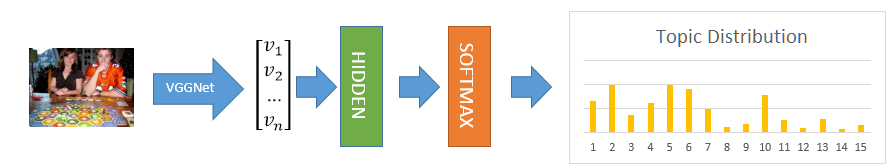
\includegraphics[width=\textwidth]{LDANetwerktranslate.png}
		\caption{Overview of LDA topic distribution prediction for an unseen image}
		\label{fig:ldaprocess}
	\end{figure*}
	
	\subsection{CCA-Based Information}
	Since Jia et al.~\cite{Fernando2015} propose CCA as a method to extract semantic information from images, we follow their approach to compare the performance of CCA with our own LDA additions. CCA focuses in finding correlations between the image and sentence representations. The projection is based on the image vectors computed with VGGNet and a term frequency-inverse document frequency (tf-idf) weighted vector representation for the descriptions. We use the CCA projection of the image with 256 dimensions as experiments show this performs best. 
	
	All sentences are considered on their own, to make sure all different descriptions are maximally correlated to the corresponding image. The LDA approach described above considers the five sentences as a whole, because the goal is to learn a topic distribution based on the image. All five descriptions should thus be considered as sampled from the same topic distribution.
	
	
	\subsection{Adding Information to RNN}
	The LDA topic distribution can guide the RNN generation process. The topic distribution $L$, predicted by the neural network described in section~\ref{sec:LDAinfo} is integrated using formulas~\eqref{eq:rnnstart}-\eqref{eq:rnnend}. The elements in red are our contributions to the original formulas proposed by Karpathy et al.~\cite{Karpathy2015}. $W_{hi}, W_{hx}, W_{hh}, W_l, b_h$ and $b_v$ are parameters to be learned by the network. $x_t$ and $y_t$ are the in- and output at time $t$. $h_t$ are the values of the hidden layer at time $t$. $CNN_{\theta_c}(I)$ is the output of VGGNet given image $I$. $f$ is an activation function.
	
	\begin{align}
	\vspace{-3mm}
	\label{eq:rnnstart}
	b_v&=W_{hi} [CNN_{\theta_c}(I)] \\
	\label{eq:rnn}
	h_t&=f(W_{hx} x_{t} + W_{hh} h_{t-1} + b_h + b_v \color{red}{+W_lL}\color{black}) \\
	y_t&=Softmax( W_{oh} h_t + b_o)
	\label{eq:rnnend}
	\end{align}
	
	
	
	\subsection{Adding Information to LSTM}
	The addition of semantic information to the LSTM network of Vinyals et al.~\cite{Google} follows the gLSTM approach of Jia et al.~\cite{Fernando2015}. They propose four different guides of which the CCA projections produce the best results. We experiment with both LDA and CCA based vectors containing semantic information.
	
	\subsection{Normalizing Beam Search}
	Since the beam search implementation focuses on maximizing the log probability of the generated sentence, the algorithm favors shorter sentences. To cope with this, Jia et al.~\cite{Fernando2015} propose a normalization function. They propose a Gaussian function based on the sentence length distribution of the training set. We add the use of $idf$ weights as another possible normalization. Formula~\eqref{eq:log-sentence-norm} shows how this function $\Omega(\ell)$ is added to the beam search probability. $\ell$ is the length of the current word sequence. $x_i$ is the $i$th word in the sequence, $I$ is the image and $\zeta$ represents the parameters of the language model. 
	
	\begin{equation}
	p = \frac{1}{\color{red}{\Omega(\ell)}}\sum_{i=1}^{\ell} \log p(x_i | I, x_{1:i}, \zeta)
	\label{eq:log-sentence-norm}
	\end{equation}
	
	The Gauss normalization implements the normalization as the value of the Gaussian distribution based on the sentence lengths of the training corpus. This leads to $\Omega(\ell) \sim \mathcal{N}(\mu, \sigma)$ with $\mu$ and $\sigma$ the average and standard deviation of the sentence length. This forces the length of the generated sentences to be similar to the length of the training sentences.
	
	Our own contribution focuses on the quality of the generated sentences. These sentences seem to prefer vague terms, leading to higher BLEU scores and sentences that are often too general. To solve this, we implement the $\Omega$ function based on the idf weights of the individual words in the training set. Summing these weights over all words in a sentence gives an estimate of how much ``information'' the sentence contains. Doing so, sentences that use only frequent words are punished. This normalization also gives higher probabilities to longer sentences. Formula~\eqref{eq:idfnorm} contains the exact calculation of this score. $N$ is the total number of training images, and $n_i$ is the number of training sentences the $i$th word of the generated sentence occurs in.
	
	\begin{equation}
		\Omega(\ell) = \sum_{i=1}^{\ell}\log(\frac{N}{n_i})
		\label{eq:idfnorm}
	\end{equation}

	\subsection{Introducing Noise}
	\label{sec:noise}
	To evaluate the ability of the gLSTM to deal with noisy training data, we add noise to the training set in the following way. The main purpose of this is to compare both semantic guides on how resistant they are to random noise. The noise is introduced as follows. Each word in the training sentences is replaced with another, random word with a probability of 0.15.
	
	\section{Experiments}
	\label{sec:exp}
	\subsection{Dataset}
	For evaluation and training we use \emph{Flickr30k}~\cite{Young2014}. Flickr30k is a widely adopted dataset containing images together with five reference captions. We use the publicly available splits~\cite{Karpathy2014} that divide the set into 28,000 images for training, 1,000 for testing and 1,000 for validating. 
	
	\subsection{Evaluation Metrics}
	To evaluate the models we follow the current literature and document the two most popular automatic evaluation metrics: BLEU~\cite{Papineni2002} and Meteor~\cite{Denkowski2007a}. BLEU is a form of precision of word $n$-grams between generated and reference sentences. Unlike the original paper we follow Jin et al.~\cite{Jin2015} and drop the brevity penalty to be able to compare. BLEU has some obvious drawbacks such as the requirement of exact word matches. Elliott et al.~\cite{Elliott2014} show that the lower BLEU scores correlate weakly with human evaluation. Meteor and the higher BLEU scores achieve moderate correlation. Meteor tries to solve some of the drawbacks of BLEU by including recall, synonyms, stemming and phrase table matches.
	
	In addition to the automatic evaluation measures we also look at some other statistics of the generated systems to evaluate the creativity and quality of the generated sentences.
	Interesting metrics include the sentence length, vocabulary size, word usage and the number of unique sentences.
	
	\subsection{Implementation Details}
	
	Our implementation extends the code publicly available by Karpathy\footnote{\url{https://github.com/karpathy/neuraltalk}}.
	Since we do not evaluate BLEU scores with a brevity penalty and Karpathy~\cite{Karpathy2015} does not provide a Meteor score, we define a set of default settings and create a reference model with his RNN implementation.
	To be able to compare with the results of Vinyals et al.~\cite{Google} we also create a reference model with the provided LSTM implementation.
	
	We use the last fully-connected layer of the 16-layer VGGNet~\cite{Arge2015} convolutional neural network pre-trained on ImageNet~\cite{Russakovsky2014} as an image representation.
	The default training settings use \emph{RMSprop}~\cite{RMSprop} with batches of 100 images, a decay rate of 0.999, epsilon smoothing factor 1e-8 and an initial learning rate of 1e-4. The network has 256 hidden units and an image and word encoding of size 256.
	To reduce the effect of exploding gradients and overfitting we use gradient clipping with threshold 5 and a drop-out percentage of 50 respectively.
	Only words that occur more than 5 times in the training set are added to the vocabulary. For testing we use a beam-length of 50.
	Due to time constraints we do not experiment with other settings.
	
	Just like the original paper by Jia et al.~\cite{Fernando2015}, we implement the gLSTM on top of the LSTM code by Karpathy.
	For both LDA and CCA we first stem the words with the publicly available Natural Language ToolKit (NLTK)\cite{bird2009natural}.
	We use the \emph{canoncorr} function available in \texttt{MATLAB} to compute the CCA projection matrices. We experiment with different numbers of correlation components but find that 256 provides the best results.
	We learn an LDA model with the \emph{python} package \emph{lda}\footnote{\url{https://pypi.python.org/pypi/lda}}. 
	Experiments with different numbers of topics show that the gLSTM benefits the most from 120 topics.
	
	
	\subsection{Results}
	\paragraph{Adding information to RNN}
	Karpathy~\cite{Karpathy2015} states that results improve by adding the image only at the first generation step. Our reference add the image each time step, but we found the results to be comparable to the original. We did consider adding the image only once with LDA. This does not improve the results however.
	Table~\ref{table:results_rnn} compares the scores of the reference to those of a system with LDA. It also shows that the reference (\emph{ref-RNN}, feeding the image each time step and not using LDA) approximates the results of the original paper by Karpathy after application of the brevity penalty to the BLEU scores. 
	It is clear that the addition of LDA improves the results on all considered metrics.
	
	\begin{table}
		\centering
		\begin{tabular}{lllllll}
			& B1 & B2 & B3 & B4 & M \\ \hline
			Karpathy$^*$~\cite{Karpathy2015}    & 57.3   & 36.9   & 24     & 15.7   & ~           \\    
			ref-RNN$^*$     & 55.2   & 36.6   & 23.9   & 15.1   & 14.3          \\
			ref-RNN          & 64.9  & 43.1     & 28.1   & 17.8   & 14.3          \\
			RNN + LDA         & \textbf{65.4}   & \textbf{44}     & \textbf{29.1}   & \textbf{19}     & \textbf{14.4}          \\\hline
		\end{tabular}
		\caption{Comparison of results of adding LDA to RNN with reference and original paper~\cite{Karpathy2015} on Flickr30k. $^{*}$ indicates results with brevity penalty. B$n$ is the BLEU-$n$ score. M is the Meteor score.}
		\label{table:results_rnn}
	\end{table}
	
	\paragraph{Adding Information to LSTM}
	Table~\ref{table:results_lstm} shows the effect of adding a semantic guide to the LSTM. Both guides considered improve the results on the most important metrics compared to the reference (\emph{ref-LSTM}) and the original paper. LDA scores best on Meteor while CCA is the best performer on the high BLEU metrics. Compared to RNN, LSTM produces slightly longer sentences, uses more unique words and generates more unique sentences.
	\begin{table}
		\centering
		\begin{tabular}{lllllll}
			& B1 & B2 & B3 & B4 & M \\ \hline
			Vinyals~\cite{Google}      & \textbf{66.3}   & 42.3   & 27.7   & 18.3   & ~     \\ 
			ref-LSTM         & 62.1   & 41.4   & 27.1   & 17.6   & 15.1  \\
			gLSTM+LDA         & 64.4   & \textbf{43.2}   & 28.1   & 17.8   & \textbf{16}  \\
			gLSTM+CCA         & 63.7   & 43.4   & \textbf{29.2}   &\textbf{19.3}   & 15.8  \\ \hline
		\end{tabular}
		\caption{Comparison of results of adding LDA and CCA to LSTM with reference and original paper on Flickr30k. B$n$ is the BLEU-$n$ score. M is the Meteor score.}
		\label{table:results_lstm}
	\end{table}
	
	
	\paragraph{Normalizing Beam Search}
	We experiment with two normalization strategies. First we look at the effects of Gauss normalization. The goal of this strategy is to generate longer sentences with higher quality. Table~\ref{table:results_gauss} shows that Gauss normalization always improves the Meteor score. For most of the models except for gLSTM with CCA it also improves BLEU-3 and BLEU-4. Jia et al.~\cite{Jia2014} point out that the lower BLEU scores have the bad property to favor shorter sentences. Therefore Gauss normalization does not improve BLEU-1 and BLEU-2.
	
	\begin{table}
		\centering
		\begin{tabular}{lllllll}
			& B1 & B2 & B3 & B4 & M \\ \hline
			ref-RNN          & \textbf{64.9}  & \textbf{43.1}     & 28.1   & 17.8   & 14.3          \\
			RNN$^+$       & 62.4   & 42     & \textbf{28.2}   & \textbf{18.6}   & \textbf{16.6}          \\ \hline
			RNN+LDA         & \textbf{65.4}   & \textbf{44}     & \textbf{29.1}   &19     & 14.4 \\
			RNN+LDA$^+$ & 62.7   & 42.6   & 28.8   & \textbf{19.5}   & \textbf{16.6}           \\ \hline 
			ref-LSTM         & \textbf{62.1}   & \textbf{41.4}   & 27.1   & 17.6   & 15.1  \\
			LSTM$^+$        & 61.2   & 41.1   & \textbf{27.3}   & \textbf{18.2}   & \textbf{16.9}  \\ \hline
			gLSTM+LDA         & \textbf{64.4}   & \textbf{43.2}   & 28.1   & 17.8   & 16  \\
			gLSTM+LDA$^+$ & 62.7   & 42.5   & \textbf{28.8}   & \textbf{19.4}   & \textbf{17.4}  \\\hline
			gLSTM+CCA         & \textbf{63.7}   & \textbf{43.4}   & \textbf{29.2}   &\textbf{19.3}   & 15.8  \\
			gLSTM+CCA$^+$ & 62.1   & 41.9   & 28.2   & 18.7   & \textbf{17.2}  \\\hline
		\end{tabular}
		\caption{Effect of adding Gauss normalization evaluated on Flickr30k. $^+$ indicates the use of Gauss normalization. B$n$ is the BLEU-$n$ score. M is the Meteor score.}
		\label{table:results_gauss}
	\end{table}
	
	Gauss normalization also achieves its second goal. The length of the sentences grows from an average of 7.5 to 10.3 words. The number of generated sentences that are not in the training set grows from 75\% to 90\%. The number of truly unique sentences (not occurring in the training set and only occurring once in the generated sentences) does not show this growth. Figure~\ref{fig:gauss} shows an example of how Gauss normalization leads to a better description.
	
	\begin{figure}
		\centering
		\begin{minipage}[t]{.45\textwidth}
			\centering
			\vspace{0pt}
			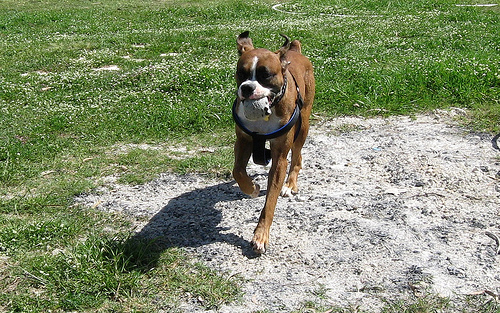
\includegraphics[width=\textwidth]{Images/hond}
		\end{minipage}\hfill	
		\begin{minipage}[t]{.7\textwidth}
			\vspace{0pt}
			\begin{tabular}{ll}
				gLSTM & \texttt{A dog runs through the grass} \\
				gLSTM+Gauss & \texttt{A brown and white dog is}\\
				~ & \texttt{running through the grass} \\
			\end{tabular}
		\end{minipage}
		\caption{Example of improvement made by Gauss normalization.}
		\label{fig:gauss}
	\end{figure}
	
	As a second normalization strategy we propose idf normalization. We evaluate this normalization on the gLSTM model with LDA as guide. The goal is to generate longer sentences that also contain more information. Because this normalization favors more unseen words, we expect the BLEU score to drop significantly. A manual evaluation of the generated sentences shows that most images indeed lead to longer, more humanlike sentences that use less generic words. On the other hand a lot of the generated descriptions contain unwanted word repetitions and sentences that no longer correspond to the image.
	
	Table~\ref{table:results_idf} shows the automatic evaluation measures of idf normalization. The BLEU scores deteriorate dramatically, the Meteor score also decreases. Table~\ref{table:idf-stats} displays other interesting statistics that show that the idf normalization increases the creativity of the language model and creates longer sentences. Idf normalization generates sentences with an average length of 10.5. Figure~\ref{fig:idf} shows an example of an improved caption and a caption where the system fails.
	
	\begin{table}
		\centering
		\begin{tabular}{llllll}
			~                  & B1 & B2 & B3 & B4 & M \\ \hline
			gLSTM        & 64.4   & 43.2            & 28.1   & 17.8   & 16 \\
			gLSTM+idf   & 40.7   & 23.2   & 13.4   & 7.6 & 12.8 \\ \hline
			
		\end{tabular}
		
		\caption{Effects of adding idf-normalization evaluated on Flickr30k. B$n$ is the BLEU-$n$ score. M is the Meteor score.}
		\label{table:results_idf}
	\end{table}
	
	\begin{figure}
		\centering
		\begin{minipage}[t]{.45\textwidth}
			\centering
			\vspace{0pt}
			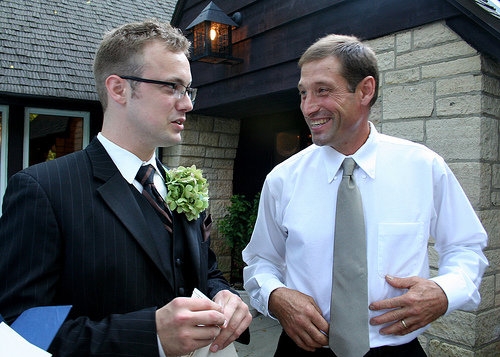
\includegraphics[width=\textwidth]{Images/trouw}
		\end{minipage}\hfill	
		\begin{minipage}[t]{.7\textwidth}
			\vspace{0pt}
			\begin{tabular}{ll}
				gLSTM & \texttt{A man and woman are talking} \\ 
				~ & \texttt{to each other} \\
				gLSTM+idf & \texttt{Two men dressed in formal}\\
				~ & \texttt{attire share a conversation} \\
			\end{tabular}
		\end{minipage}
		\centering
		\begin{minipage}[t]{.45\textwidth}
			\centering
			\vspace{0pt}
			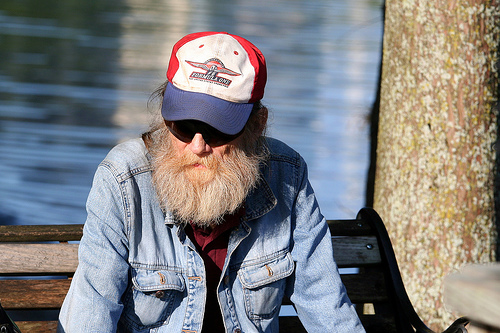
\includegraphics[width=\textwidth]{Images/441817653}
		\end{minipage}\hfill
		\begin{minipage}[t]{.7\textwidth}
			\vspace{0pt}
			\begin{tabular}{ll}
				gLSTM & \texttt{A man in a black jacket is} \\ 
				~ & \texttt{looking at the camera} \\
				gLSTM+idf & \texttt{African american african}\\
				~ & \texttt{american male wearing a blue} \\
				~ & \texttt{jacket is looking at the} \\
				~ & \texttt{camera} \\
			\end{tabular}
		\end{minipage}
		\caption{Examples of better and worse results with idf normalization.}
		\label{fig:idf}
	\end{figure}
	
	\begin{table*}
		\centering
		\begin{tabular}{llllll}
			~                   & Unique words& Avg Sentence Length & Unique1 & Unique2 \\ \hline
			gLSTM                         & 296   & 8.33   & 775   & 490  \\
			
			gLSTM+idf                 & \textbf{721}   & \textbf{10.5}   & \textbf{991}   & \textbf{927}    \\\hline
		\end{tabular}
		\caption{Effects of adding idf-normalization to gLSTM with LDA on the sentence statistics. \emph{Unique1} is the number of sentences not occurring in the training set. \emph{Unique2} is the amount of sentences that are only generated once and do not occur in the training set.}
		\label{table:idf-stats}
	\end{table*}
	
	\paragraph{Noise Resistance}
	As a last experiment we evaluate gLSTM on the noisy training set (section~\ref{sec:noise}) with both LDA and CCA as guide.
	Table~\ref{table:noisy} shows the results. Both LDA and CCA only show a small drop in the evaluation results. They are still able to generate gramatically correct sentences. A manual inspection of the most important words in each topic of LDA shows that they still are logically connected. A possible explanation of this ability to deal with noise is the way both of the models train. They both use data from 5 training sentences. The probability that all these 5 sentences show the same errors is small. Further experiments with more word changes in the sentences and other types of noise seem necessary to understand the full extent of their robustness.
	
	\begin{table}
		\centering
		\begin{tabular}{lllllll}
			~                  & B1 & B2 & B3 & B4 & M \\ \hline
			LDA   & 64.4   & 43.2   & 28.1   & 17.8 & 16 \\
			LDA+noise   & 63.8   & 42.6   & 27.9   & 18.2 & 15.8\\ \hline
			CCA   & 63.7   & 43.4   & 29.2   & 19.3 & 15.8 \\
			CCA+noise   & 63.4  & 42.7   & 28.6   & 18.8 & 15.5 \\ \hline			
		\end{tabular}
		\caption{Effect of noise on the automatic evaluation criteria for LDA and CCA as guide for gLSTM. B$n$ is the BLEU-$n$ score. M is the Meteor score.}
		\label{table:noisy}
	\end{table}
	
	
	
	\paragraph{Comparison with Literature}
	Table~\ref{tab:sota} compares our best results with the results reported in the most recent literature. We compare our systems with Vinyals~\cite{Google} since we extend the model that they propose. We also look at Jia et al.~\cite{Fernando2015} since they proposed the gLSTM model we implemented. We also include the results of two attention based systems~\cite{Jin2015, Xu2015}. 
	
	The current systems still have a few recurring problems. The models often connect colors with a wrong object. Numbers of objects form a second difficulty. LDA is not able to help with this problem since it contains a topic of numbers. It does help a bit with colors since it combines similar colors into topics.
	
	During the experiments, we left a lot of training parameters untouched, since training a network took roughly a week on the provided hardware. Tuning these parameters may lead to improved results. This is probably why the results of Jia et al.~\cite{Fernando2015} using CCA are better than our own implementation. However, our results are comparable with theirs. 
	
	The attention models perform best. It seems promising to extend our models with attention vectors. Adding attention to a model makes the training more complex and slower. This is why our RNN+LDA model is still good competition for the attention based models. The results are quite close, and our network is much faster to train. 
	
	\begin{table}
		\centering
		\begin{tabular}{llllll}
			~                  & B1 & B2 & B3 & B4 & M \\ \hline
			RNN+LDA            & \textbf{65.4}   & \textbf{44}     & 29.1   & 19     & 14.4  \\
			RNN+LDA$^+$      & 62.7   & 42.6   & 28.8   & \textbf{19.5}   & 16.6  \\
			gLSTM+LDA$^+$    & 62.7   & 42.5   & 28.8   & 19.4   & \textbf{17.4}   \\
			gLSTM+CCA          & 63.7   & 43.4   & \textbf{29.2}   & 19.3   & 15.8  \\ \hline
			Vinyals~\cite{Google}           & 66.3   & 42.3   & 27.7   & 18.3   & ~      \\
			Jia~\cite{Fernando2015}  & 64.6   & 44.6   & 30.5   & 20.6   & 17.9  \\
			Xu~\cite{Xu2015}     & 66.9   & 43.9   & 29.6   & 19.9   & 18.5  \\
			Jin~\cite{Jin2015}      & \textbf{67}    & \textbf{47.5}   & \textbf{33}     & \textbf{24.3}   & \textbf{19.4}   \\ \hline
		\end{tabular}
		\caption{Comparison of our best results with the current state of the art. $^+$ indicates the use of Gauss normalization. B$n$ is the BLEU-$n$ score. M is the Meteor score.}
		\label{tab:sota}
	\end{table}
	
	\section{Conclusion}
	This contribution tries to improve existing image description systems. Extensions are made by adding semantic information using LDA and CCA, and with a normalization factor in the beam search algorithm.
	
	Adding LDA topic distributions as additional information to the RNN implementation described by Karpathy~\cite{Karpathy2015} improves the results on all metrics. It should be noted that RNN trains faster than the LSTM implementation but achieves comparable results. For now we used 120 topics, but further research on the upper limit of this number may lead to a bigger improvement.
	
	Extending the LSTM model proposed by Vinyals~\cite{Google} with both considered semantic guides leads to better results. LDA yields better Meteor scores, while CCA increases the BLEU scores. Compared to the original gLSTM paper~\cite{Fernando2015} our system performs slightly worse. Most of the parameters of our network were not fine tuned during training. Further research of the effect of these parameters may lead to improvement.
	
	Using Gauss normalization improves BLEU-3, BLEU-4 and Meteor scores. It also leads to longer sentences. The number of generated sentences that are not in the training set increases drastically. A gLSTM model with LDA as guide and Gauss normalization achieves the best results on the scores that correlate best with human evaluation. Idf normalization does not lead to better BLEU and Meteor scores, since it focuses on words that are not used frequently. It does however lead to more creative sentences. Apart from a lot of improved sentences it sometimes forces the model to diverge from the image content or add word repetitions. Investigating possible ways to tune the idf normalization function may lead to sentences that are both creative and correct descriptions of the image.
	
	A comparison of the two semantic guides on their noise resistance shows that they are both very resistant. Both the BLEU and Meteor scores decrease only slightly This is probably caused by the training with 5 reference sentences. Other experiments with more changed words and other types of noise are necessary to understand the full extent of this robustness.
	
	This work produces results comparable to the literature. Attention based models still outperform our models so adding attention can perhaps further improve our results.
	
	%----------------------------------------------------------------------------------------
	%	REFERENCE LIST
	%----------------------------------------------------------------------------------------
	
	\bibliographystyle{abbrv}
	\bibliography{referenties,extra_references}
	
	%----------------------------------------------------------------------------------------
	
	\clearpage
	\appendix
	\section{LDA prediction}
	\label{appendix:LDA}
	\subsection{Choosing the number of topics}
	The number of topics is the most important parameter of an LDA model. However, it is a nontrivial task to evaluate the quality of such a model. This makes it hard to find the perfect number of topics. Since Jin et al.~\cite{Jin2015} propose 80 topics, we experiment with numbers in this range.
	
	To get a grip on the accuracy of the trained LDA model, we manually evaluate the learned topic distributions. The ten most probable words for each topic give a global idea of how coherent the topics are. For each topic a summarizing name is chosen. Table~\ref{tbl:woorden-naar-topic} gives two examples of these chosen names.
	
	Experiments show that when training a model with less than 50 topics, it becomes very difficult to find topic names that capture the learned concepts. When going higher than 120, each concept is captured in many topics, which might make it very hard for the language model to distinguish between them. It also leads to longer computation times. 
	
	\begin{table*}[!t]
		\centering
		\begin{tabular}{ll}
			Most probable words                                               & Topic Name \\ \hline
			\texttt{\small{wave man surf ocean surfer ride surfboard person wetsuit board}} & \texttt{surfing}       \\
			\texttt{\small{car truck drive vehicl back van road park driver behing}}        & \texttt{vehicle}      \\
		\end{tabular}
		\caption{Most probable stemmed words together with chosen topic name}	\label{tbl:woorden-naar-topic}
	\end{table*}
	
	\subsection{Topic distribution predictions}
	As described in section~\ref{sec:LDAinfo} our approach uses a simple feedforward neural network to predict the topic distributions for unseen images. This section shows some prediction results. For each shown image, the five most probable topic names are displayed. Figure~\ref{fig:predcorrect} shows predictions that are correct. Figure~\ref{fig:predsemi} shows predictions where the network makes small mistakes, but most of the topics are correct. Figure~\ref{fig:predwrong} shows images where the network is mistaken about the contents of the image. Moreover we find that these images correspond to those that are described poorly by each of the investigated systems. This might be caused by a bad image representation.
	
	
	\begin{figure*}
		\begin{subfigure}{\textwidth}
			\centering
			\begin{minipage}[t][4cm]{.5\linewidth}
				\centering
				\vspace{0pt}
				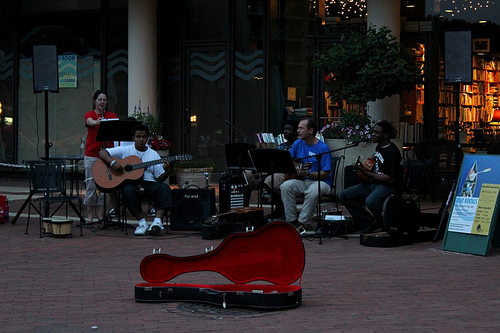
\includegraphics[height=4cm]{Images/4691655601.jpg}
			\end{minipage}\hfill
			\begin{minipage}[t]{.5\textwidth}
				\centering
				\vspace{0pt}
				\begin{tabular}{cl}
					Topic                           & Probability\\
					\hline
					\texttt{sit outside}             & 0.095 \\
					\texttt{sit/chair}                   & 0.070 \\
					\texttt{musicians}                 & 0.047 \\
					\texttt{instruments}           & 0.035 \\
					\begin{tabular}{c}
						\texttt{sit at table/}\\
						\texttt{restaurant}
					\end{tabular}       & 0.032\\
					\hline
				\end{tabular}
			\end{minipage}
		\end{subfigure}
		\vspace*{4mm}
		\begin{subfigure}{\textwidth}
			\centering
			\begin{minipage}[t][4cm]{.5\linewidth}
				\centering
				\vspace{0pt}
				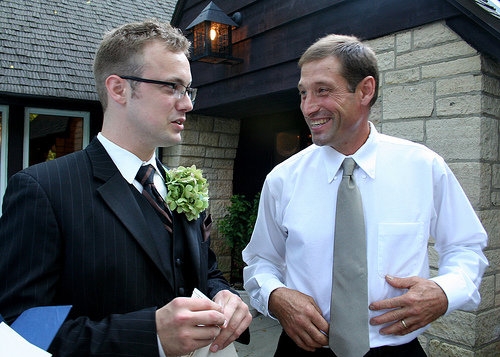
\includegraphics[height=4cm]{Images/2773744784.jpg}
			\end{minipage}\hfill
			\begin{minipage}[t]{.5\textwidth}
				\centering
				\vspace{0pt}
				\begin{tabular}{cl}
					Topic                           & Probability\\
					\hline
					\texttt{formal clothing}             & 0.110 \\
					\texttt{men together}                   & 0.078 \\
					\texttt{couple/wedding}                 & 0.062 \\
					\texttt{older man}           & 0.058 \\
					\texttt{beard/mustache}        & 0.041\\
					\hline
				\end{tabular}
			\end{minipage}
		\end{subfigure}
		\caption{Images with the five most probable topics, correct prediction}
		\label{fig:predcorrect}
	\end{figure*}
	
	\begin{figure*}
		\begin{subfigure}{\textwidth}
			\centering
			\begin{minipage}[t][4cm]{.5\linewidth}
				\centering
				\vspace{0pt}
				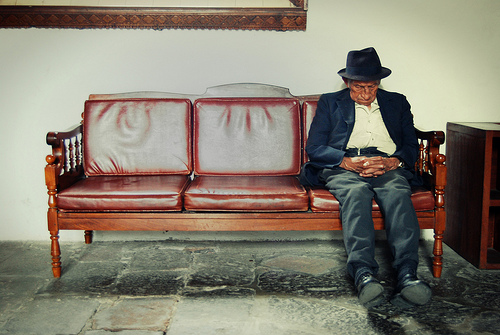
\includegraphics[height=4cm]{Images/4862204000.jpg}
			\end{minipage}\hfill
			\begin{minipage}[t]{.5\textwidth}
				\centering
				\vspace{0pt}
				\begin{tabular}{cl}
					Topic                           & Probability\\
					\hline
					\texttt{sit/chair}             & 0.044 \\
					\texttt{sit outside}                   & 0.041 \\
					\texttt{dog}                 & 0.036 \\
					\texttt{room/floor}           & 0.031 \\
					\texttt{sleep/laydown}        & 0.027\\
					\hline
				\end{tabular}
			\end{minipage}
		\end{subfigure}
		\vspace*{4mm}
		\begin{subfigure}{\textwidth}
			\centering
			\begin{minipage}[t][4cm]{.5\linewidth}
				\centering
				\vspace{0pt}
				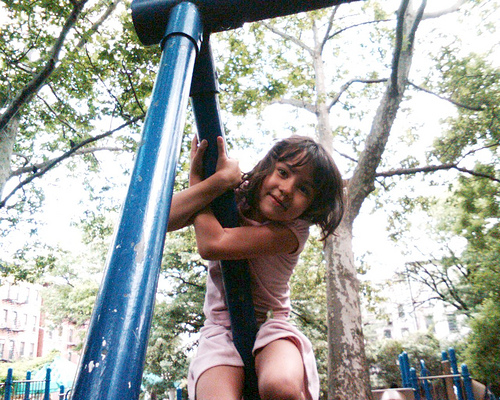
\includegraphics[height=4cm]{Images/3643021980.jpg}
			\end{minipage}\hfill
			\begin{minipage}[t]{.5\textwidth}
				\centering
				\vspace{0pt}
				\begin{tabular}{cl}
					Topic                           & Probability\\
					\hline
					\texttt{baseball}             & 0.058 \\
					\texttt{toddler}                   & 0.053 \\
					\texttt{girl}                 & 0.50 \\
					\texttt{playground}           & 0.049 \\
					\texttt{photograph}        & 0.040\\
					\hline
				\end{tabular}
			\end{minipage}
		\end{subfigure}
		\caption{Images with the five most probable topics, almost correct prediction}
		\label{fig:predsemi}
	\end{figure*}
	
	
	\begin{figure*}
		\begin{subfigure}{\textwidth}
			\centering
			\begin{minipage}[t][4cm]{.5\linewidth}
				\centering
				\vspace{0pt}
				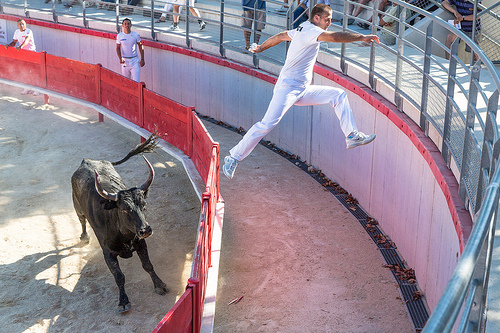
\includegraphics[height=4cm]{Images/7446693604.jpg}
			\end{minipage}\hfill
			\begin{minipage}[t]{.5\textwidth}
				\centering
				\vspace{0pt}
				\begin{tabular}{cl}
					Topic                           & Probability\\
					\hline
					\texttt{constructor}             & 0.067 \\
					\texttt{body of water}                   & 0.059 \\
					\texttt{stairs/rail}                 & 0.056 \\
					\texttt{boats}           & 0.040 \\
					\texttt{cleaning}        & 0.026\\
					\hline
				\end{tabular}
			\end{minipage}
		\end{subfigure}
		
		\vspace*{4mm}
		
		\begin{subfigure}{\textwidth}
			\centering
			\begin{minipage}[t][4cm]{.5\linewidth}
				\centering
				\vspace{0pt}
				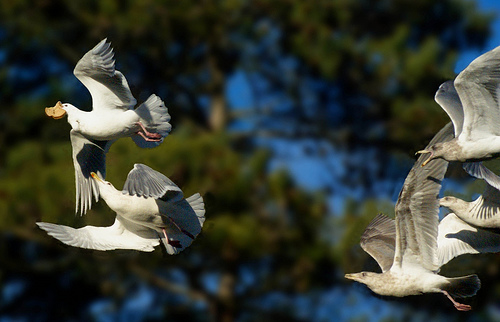
\includegraphics[height=4cm]{Images/3294830188.jpg}
			\end{minipage}\hfill
			\begin{minipage}[t]{.5\textwidth}
				\centering
				\vspace{0pt}
				\begin{tabular}{cl}
					Topic                           & Probability\\
					\hline
					\texttt{dog + toy}             & 0.077 \\
					\begin{tabular}{c}
						\texttt{shirtless/}\\
						\texttt{bird/white}
					\end{tabular}                      & 0.067 \\
					\texttt{rock climbing}                 & 0.065 \\
					\texttt{jump/trick}           & 0.034 \\
					\texttt{clothes/color}        & 0.025\\
					\hline
				\end{tabular}
			\end{minipage}
		\end{subfigure}
		
		\caption{Images with the five most probable topics, wrong prediction}
		\label{fig:predwrong}
	\end{figure*}
	
	
	
	
\end{document}
